\section{Lecture 7}

\subsection{Decoding Concatenated Codes}
Now how can we decode a concatenated code $C_{out} \diamond C{in}$ where the distance of $C_{out}$ is $D$ and that of
$C_{in}$ is $d$. Then $dist(C_{out} \diamond C_{in}) \geq Dd$. Let's try to correct $e < \frac{Dd}{2}$ errors efficiently. This would mean:
the error fraction
\[ \tau = \frac{\delta_{out}\delta_{in}}{2} \]
which is bounded away from 0 as long as the distances are. A corollary of this is an explicit, asymptotically good binary
linear code family that can efficiently correct $\tau$ errors with $\tau$ bounded away from 0.
\[ \tau(R) = \frac{\delta_{Zyablov}(R)}{2} \]
How can we decode? Let's revise what encoding was:

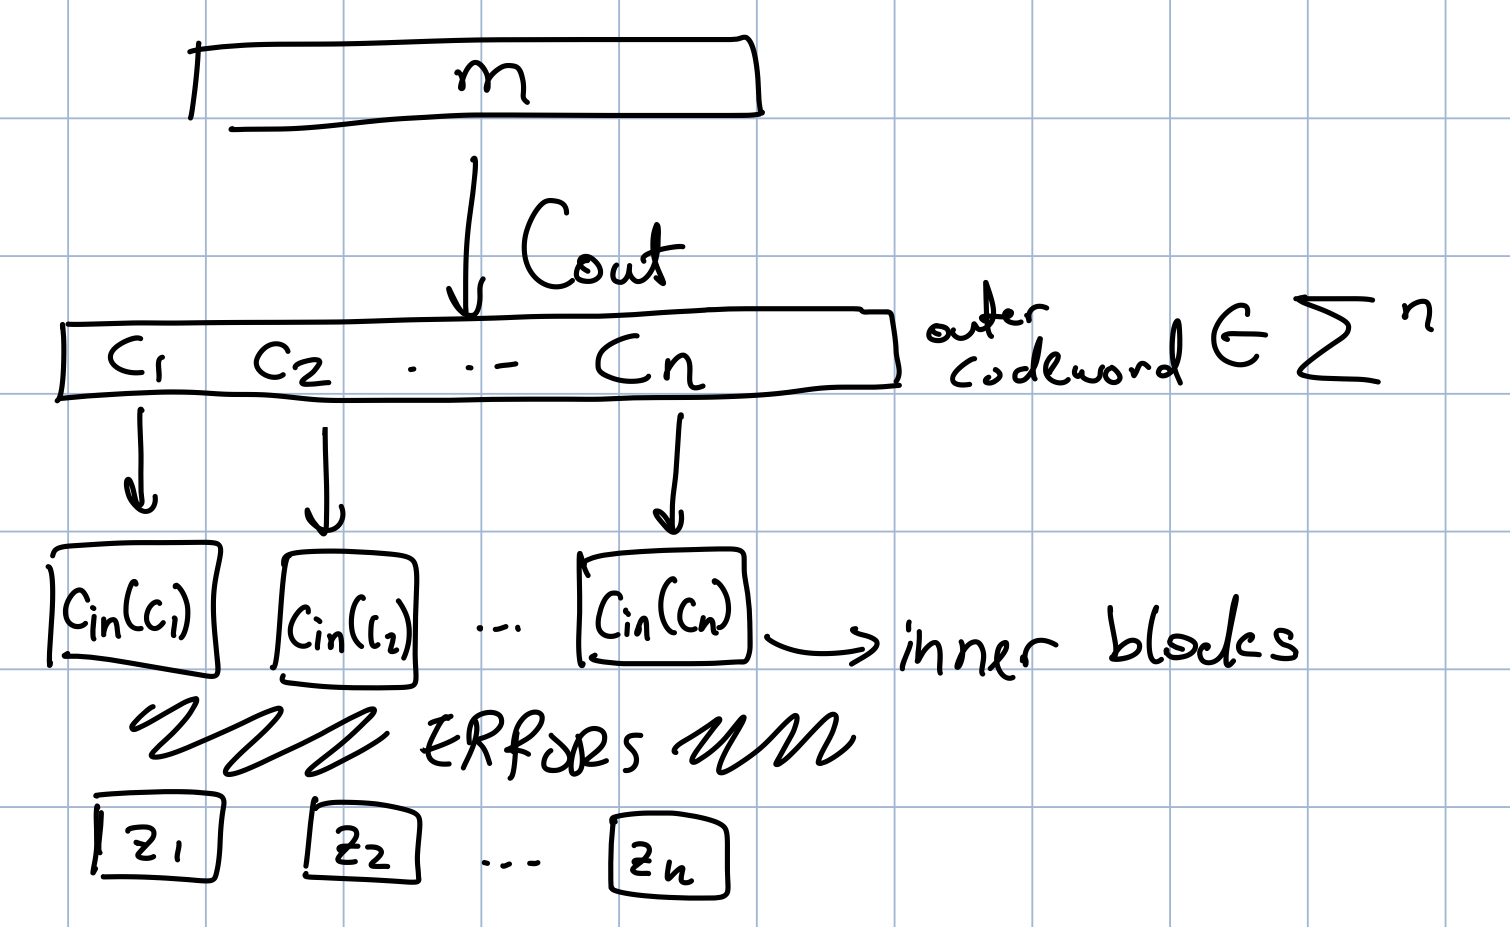
\includegraphics[width=400px]{encoder.jpeg}

Our assumption is:
\[ \sum_{i = 1}^n \Delta(z_i, C_{in}(c_i)) \leq e \]

The natural approach is to first decode the inner blocks and then decode the outer code.
\begin{enumerate}
    \item Decode each $z_i$ to $a_i \in \Sigma$ such that $\Delta(z_i, C_{in})$ is minimized (breaking ties arbitrarily). If you have a
    more efficient encoding scheme, this suffices as well.
    \item Decode $\langle a_1, a_2, \dots, a_n \rangle$ per outer decoder, up to decoding radius $D/2$.
\end{enumerate}

Runtime is efficient as long as the inner code is small, i.e. $\Sigma \leq poly(n)$. Define $N = nn'$.
\[ T(\text{outer decoder}) + n \cdot poly(|\Sigma|, n') \leq poly(N) \]

Analysis: If $|\{i \mid a_i \neq c_i \}| < \frac{D}{2}$ the algorithm suceeds. This means that if
the algo fails, then we must have $|\{i \mid a_i \neq c_i \}| \geq \frac{D}{2}$ and $a_i \neq c_i$ implies
$\Delta(z_i, C_{in}(c_i)) \geq \frac{d}{2}$. Which means that $|\{i \mid a_i \neq c_i \}| \geq \frac{D d}{4}$.
So even this simple algorithm gets within a constant factor of our desired error fraction.

Let's try a different approach. Let's have the inner decode give more guidance to outer decoder as ``soft information.''
\begin{enumerate}
    \item Decode each $z_i$ to $a_i \in \Sigma$ such that $\Delta(z_i, C_{in})$ is minimized (breaking ties arbitrarily). \textcolor{blue}{Set $w_i = \min\left\{\Delta(z_i, C_{in}(a_i)), \frac{d}{2}\right\}$}.
    \item \textcolor{blue}{For each $i$, with probability $\frac{2w_i}{d}$, erase $a_i$.} Decode $\langle a_1, a_2, \dots, a_n \rangle$ per outer decoder.
\end{enumerate}

\begin{theorem}
    If $\sum_{i = 1}^n \Delta(z_i, C_{in}(C_i)) < \frac{Dd}{2}$, then
    \[ \E{2Z_{errors} + Z_{erasures}} < D \]
    Where the $Z$ is the amount of errors/erasures in the outer code decoding.
    \begin{proof*}
        Write some indicators: $Z_{errors} = \sum Z_{errors}^i$ and $Z_{erasures} = \sum Z_{erasures}^i$.
        If $a_i = c_i$, then $Z_{errors}^i = 0$ and $\E{Z_{erasures}^{i}} = \frac{2w_i}{d} = \frac{2e_i}{d}$.
        In the other case, $\E{Z_{erasures}^i} = 2w_i/d$ and the other one is the complement.
        \begin{align*}
            \E{2 Z_{errors}^i + Z_{erasures}^i} &= 2 - \frac{2w_i}{d} \\
            &\leq 2 - \frac{2(d - e_i)}{d} \\
            &\leq \frac{2e_i}{d}
        \end{align*}
        where the second line comes from the fact that $w_i + e_i \geq d$.
        In both cases,
        \[ \E{2 Z_{errors}^i + Z_{erasures}^i} \leq \frac{2e_i}{d} \]
        which shows the claim, since $e = \sum e_i < \frac{Dd}{2}$.
    \end{proof*}
\end{theorem}

In reality, this analysis is equivalent to picking a threshold $\theta \in [0, 1]$ uniformly.
If $\theta \leq \frac{2w_i}{d}$, we declare an erasure at $i$. By this probaiblistic method,
there must exist some $\theta^*$ that makes the algorithm actually work. But, note that there are only changes in the algorithm's threshold
when $\theta$ goes between the $w_i$. Trying these $O(d)$ thresholds will get you all possibilies that matter (there are only $O(d)$ $w_i$'s).

This is called the Generalized Minimum Distance (GMD) decoding.
\subsection{Concatenation: ``Serial'' vs. ``Parallel''}
We can think of the inner codes as local codes $C_0$. With $r \ll n$ where $r = O(1)$ or $r = O(\log n)$.

% img

What if we do the following instead:

% img

We specify a set $\mathcal{F} \subseteq \binom{[n]}{r}$ (choose a subset of size $r$ under some fixed global ordering)
such that for all $S \in \mathcal{F}$, we have $c_S \in C_0$ (where $c$ is projected onto the coordinates in $S$).

Suppose we want each $i$ to belong to two local checks. Here is one such code, a product code:

% img

$n = r^2$. Then if $C_0$ is a $[r, s, d]_q$ code, then $C_0^2$ is $[r^2, s^2, d^2]_q$ code. But, rate and $\delta$ both square tho (which means they go down...).
The issue with this tensor product representation is I cannot take a local $r$ code and build a code of arbitrary size $n$.
